%% ****** Start of file apstemplate.tex ****** %
%%
%%
%%   This file is part of the APS files in the REVTeX 4.2 distribution.
%%   Version 4.2a of REVTeX, January, 2015
%%
%%
%%   Copyright (c) 2015 The American Physical Society.
%%
%%   See the REVTeX 4 README file for restrictions and more information.
%%
%
% This is a template for producing manuscripts for use with REVTEX 4.2
% Copy this file to another name and then work on that file.
% That way, you always have this original template file to use.
%
% Group addresses by affiliation; use superscriptaddress for long
% author lists, or if there are many overlapping affiliations.
% For Phys. Rev. appearance, change preprint to twocolumn.
% Choose pra, prb, prc, prd, pre, prl, prstab, prstper, or rmp for journal
%  Add 'draft' option to mark overfull boxes with black boxes
%  Add 'showkeys' option to make keywords appear
\documentclass[aps,prl,preprint,groupedaddress]{revtex4-2}
%\documentclass[aps,prl,preprint,superscriptaddress]{revtex4-2}
%\documentclass[aps,prl,reprint,groupedaddress]{revtex4-2}

% You should use BibTeX and apsrev.bst for references
% Choosing a journal automatically selects the correct APS
% BibTeX style file (bst file), so only uncomment the line
% below if necessary.
%\bibliographystyle{apsrev4-2}
\usepackage{amsmath}
\usepackage{braket}
\usepackage{float}
\usepackage{graphicx}
\usepackage{subcaption}
\begin{document}

% Use the \preprint command to place your local institutional report
% number in the upper righthand corner of the title page in preprint mode.
% Multiple \preprint commands are allowed.
% Use the 'preprintnumbers' class option to override journal defaults
% to display numbers if necessary
%\preprint{}


% repeat the \author .. \affiliation  etc. as needed
% \email, \thanks, \homepage, \altaffiliation all apply to the current
% author. Explanatory text should go in the []'s, actual e-mail
% address or url should go in the {}'s for \email and \homepage.
% Please use the appropriate macro foreach each type of information

% \affiliation command applies to all authors since the last
% \affiliation command. The \affiliation command should follow the
% other information
% \affiliation can be followed by \email, \homepage, \thanks as well.
\author{}
%\email[]{Your e-mail address}
%\homepage[]{Your web page}
%\thanks{}
%\altaffiliation{}
\affiliation{}

%Collaboration name if desired (requires use of superscriptaddress
%option in \documentclass). \noaffiliation is required (may also be
%used with the \author command).
%\collaboration can be followed by \email, \homepage, \thanks as well.
%\collaboration{}
%\noaffiliation

\date{\today}


% body of paper here - Use proper section commands
% References should be done using the \cite, \ref, and \label commands
\textbf{Key ideas}
\begin{itemize}
    \item The local energy variable $e_{loc}(s)$ is related to the derivatives of the classical network 
    \item The local variations of $e_{loc}(s)$ dictate the order of clusters one can find in the classical network derivatives
\end{itemize}



\textbf{Infinitesimal time evolution}
\begin{equation*}
    \begin{split}
    i\frac{d}{dt}\ket{\Psi(t)}&=\hat{H}\ket{\Psi(t)},\quad \Psi(s,t)=\braket{s|\Psi(t)}\\
    i\frac{d}{dt}\ket{\Psi(t)}&=\sum_s\ket{s} e_{loc}(s)\Psi(s,t),\quad e_{loc}= \frac{\braket{s|\hat{H}|\Psi(t)}}{\Psi(s,t)}
    \end{split} 
\end{equation*}
For the classical networks:
\begin{equation*}
    \begin{split}
    i\frac{d}{dt}\ket{\Psi(t)}&=\sum_{s,A}i\frac{dC_A}{dt}\chi_A(s)\Psi(s,t)
    \end{split} 
\end{equation*}
We identify:
\begin{equation}
    \begin{split}
        e_{loc}(s)= i \sum_A \frac{dC_A}{dt}\chi_A(s),\quad ||e_{loc}(s)||_2^2=\sum_A \left\lvert\frac{dC_A}{dt}\right\rvert^2
    \end{split}
\end{equation}
The last equation tells us that whenever there is a zero $|e_{loc}(s)| \rightarrow \infty$, the derivatives $C_A$ are non-holomorphic.


\textbf{Average Walsh-Hadamard order coefficients}


The discrete derivatives are defined as:

\begin{equation*}
    D_i[e_{loc}(s)]=
    \frac{e_{loc}(s)-e_{loc}(s^{\otimes i})}{2}=i\sum_{A,i\in A}\frac{dC_A}{dt}\chi_A(s)
\end{equation*}
$s^{\otimes i}=(s_1,s_2,...,-s_i,s_{i+1},...,s_N)$

The average variation or influence is:
\begin{equation*}
    Inf_i(e_{loc})=\frac{1}{2^N}\sum_s\left\lvert D_i[ e_{loc}(s)]\right\rvert^2=\sum_{A,i\in A}\left\lvert\frac{dC_A}{dt}\right\rvert^2
\end{equation*}
The total variation is:
\begin{equation*}
    \begin{split}
    \mathrm{I}(e_{loc}(s))&=\sum_i Inf_i(e_{loc}) = \sum_i \sum_{A,i\in A}\left\lvert\frac{dC_A}{dt}\right\rvert^2 \\
    \mathrm{I}(e_{loc}(s))&=\sum_A |A| \left\lvert\frac{dC_A}{dt}\right\rvert^2
    \end{split}
\end{equation*}
The average order for the coefficients is
\begin{equation}
    \langle |A|\rangle=\frac{\sum_A |A|\left\lvert\frac{dC_A}{dt}\right\rvert^2}{\sum_A \left\lvert\frac{dC_A}{dt}\right\rvert^2}=\frac{\mathrm{I}(e_{loc}(s))}{||e_{loc}||_2^2}
\end{equation}
If the local variations "($Inf_i(e_{loc})$)"  are huge, the network coefficient derivatives will include high order terms.

\textbf{\textrm{Quench Dynamics for the Ising Model}}

For our case:
\begin{equation}
    \begin{split}
    e_{loc}(s,t) &= \frac{1}{\Psi(s,t)}\sum_i \bra{s}(-Z_iZ_{i+1}-g_f X_i)\ket{\Psi(t)} \\
    e_{loc}(s,t) &= \frac{1}{\Psi(s,t)}\sum_i (-s_is_{i+1}\Psi(s,t)-g_f \Psi(s^{\otimes i},t)) \\
    e_{loc}(s,t) &= -\sum_i s_is_{i+1} -g_f \sum_i \frac{\Psi(s^{\otimes i},t)}{\Psi(s,t)} \\  
    \end{split}
\end{equation}
The variation of $e_{loc}(s,t)$ is encoded in the ratio after a spin flip $\frac{\Psi(s^{\otimes i},t)}{\Psi(s,t)}$.

\begin{figure}[H]
    \centering
    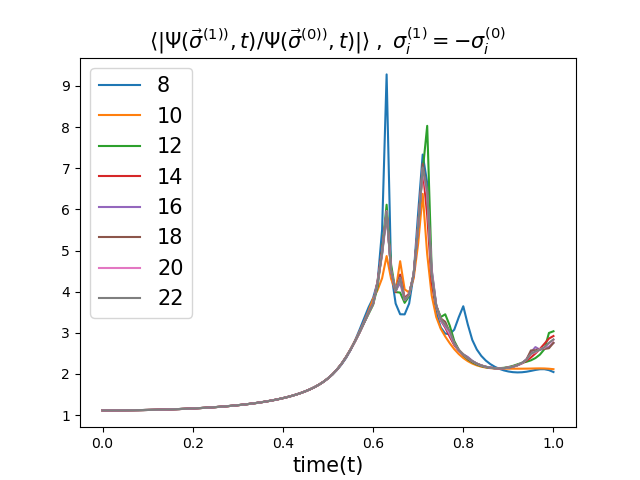
\includegraphics[width=0.8\linewidth]{figures/quench_figures/spin_flip_gi1.5_gf0.5.png}
    \caption{Average ratio for different times}
    \label{fig:1}
\end{figure}
Figure \ref{fig:1} tells us that there are states that differ in one spin flip and have drastically different 
amplitudes $\Psi(s)$. To see that in detail let us look at the histograms of the ratios:

\begin{figure}
    \centering
    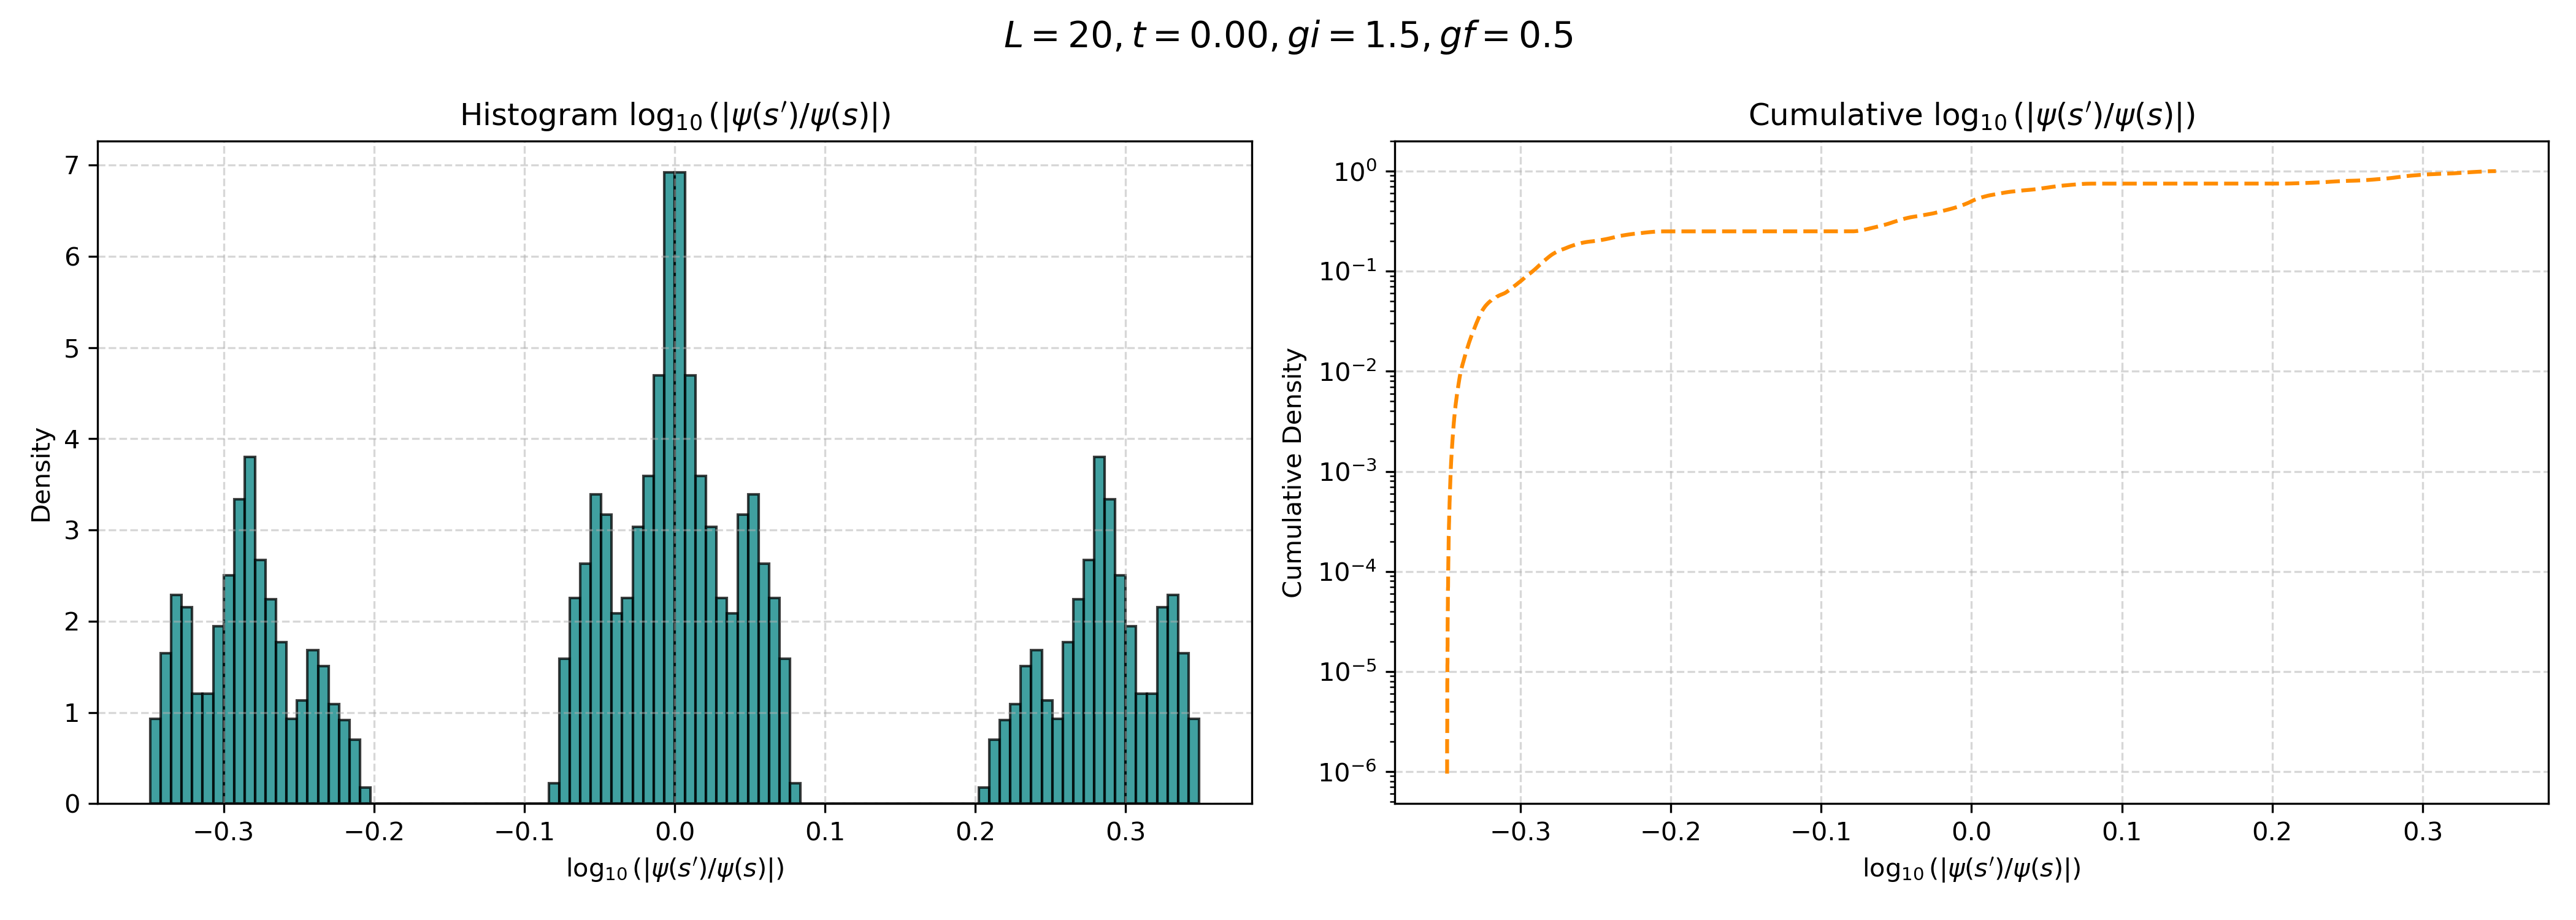
\includegraphics[width=1.0\linewidth]{figures/quench_figures/hist_plot_L20_t0_gi1.50_gf0.50.png}
    \caption{Histogram of amplitude ratios, for $t=0$. Variations are small and the amplitudes are in the same order}
    \label{fig:2}
\end{figure}
\begin{figure}
    \centering
    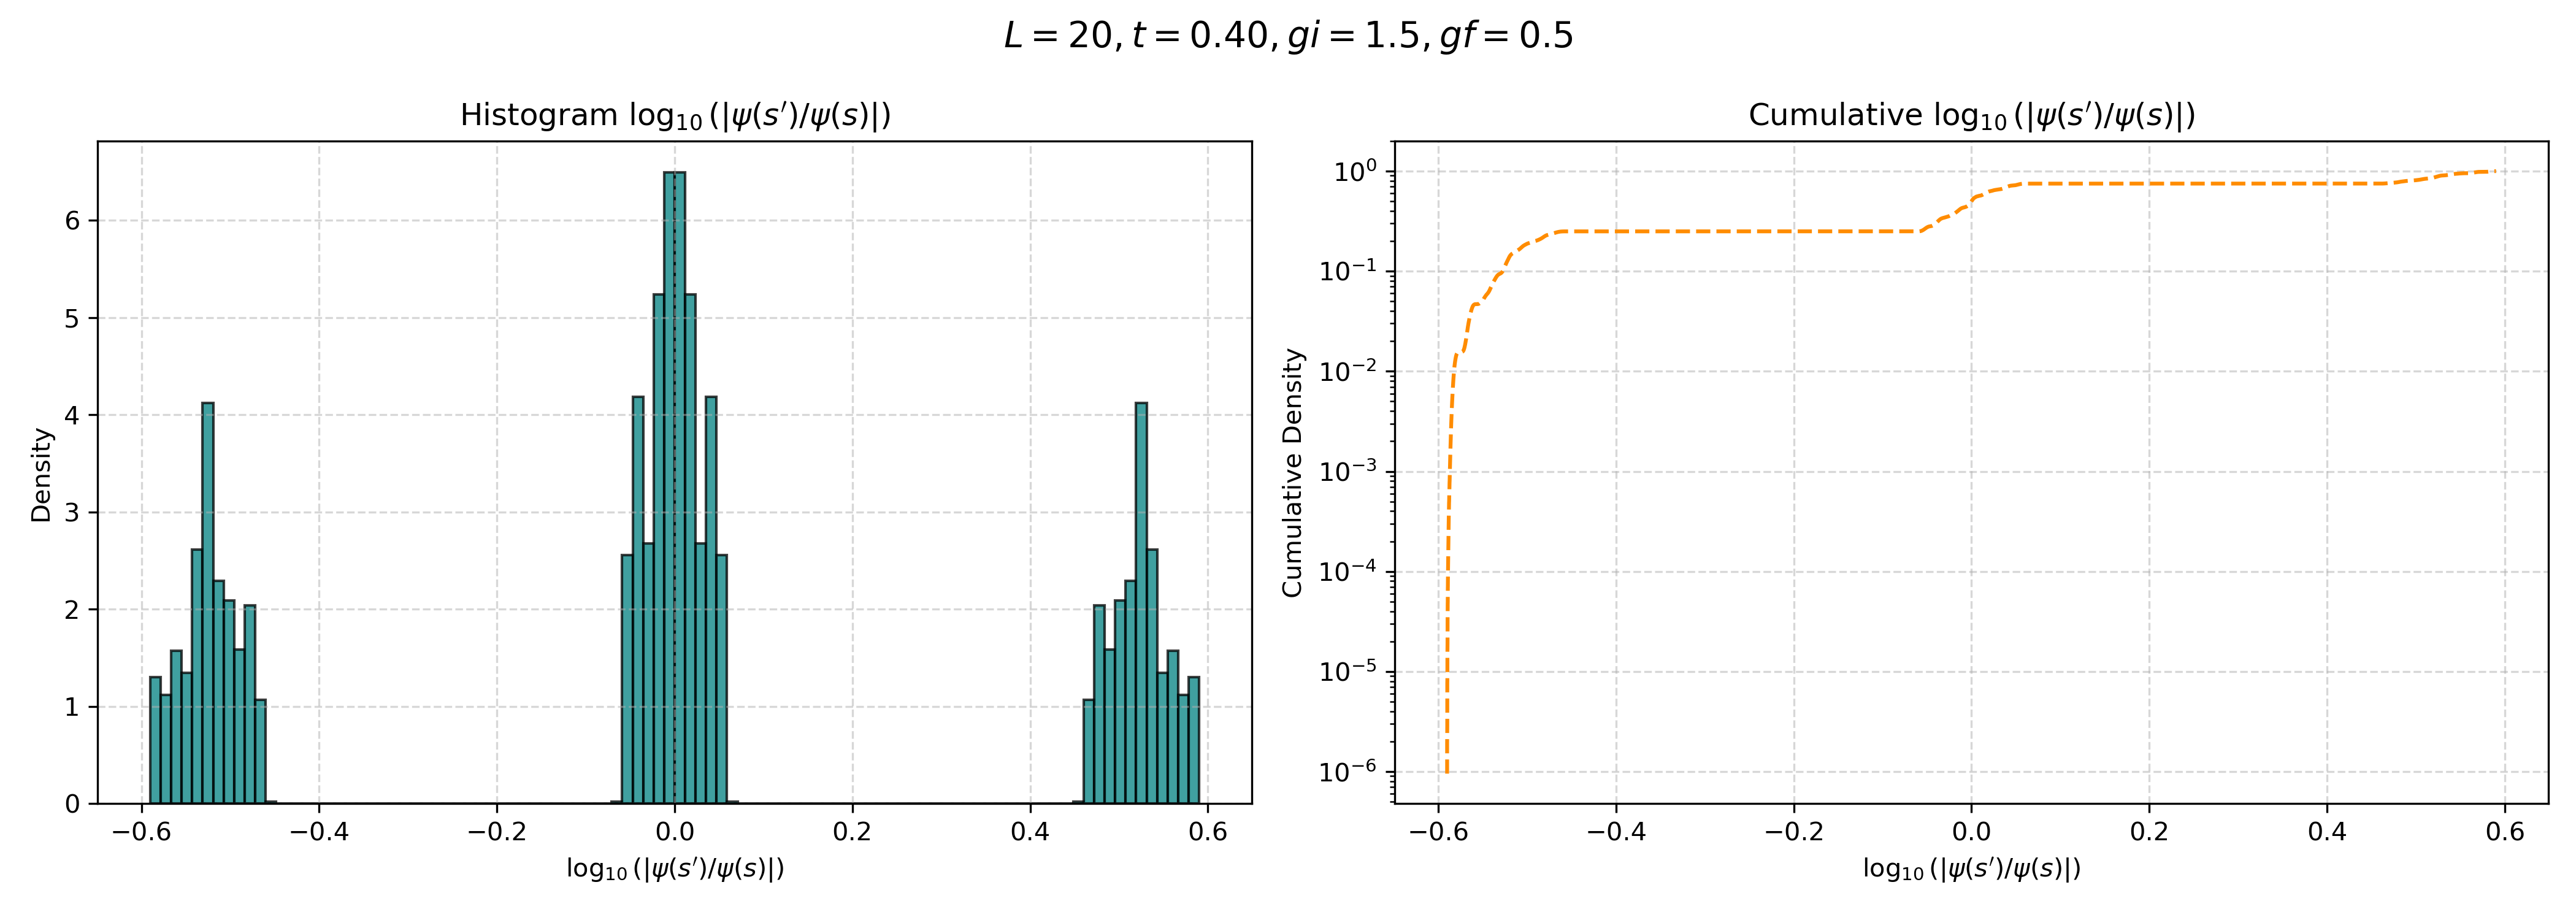
\includegraphics[width=1.0\linewidth]{figures/quench_figures/hist_plot_L20_t40_gi1.50_gf0.50.png}
    \caption{Histogram of amplitude ratios, for $t=0.4$. Amplitudes are still of the same order}
    \label{fig:3}
\end{figure}
\begin{figure}
    \centering
    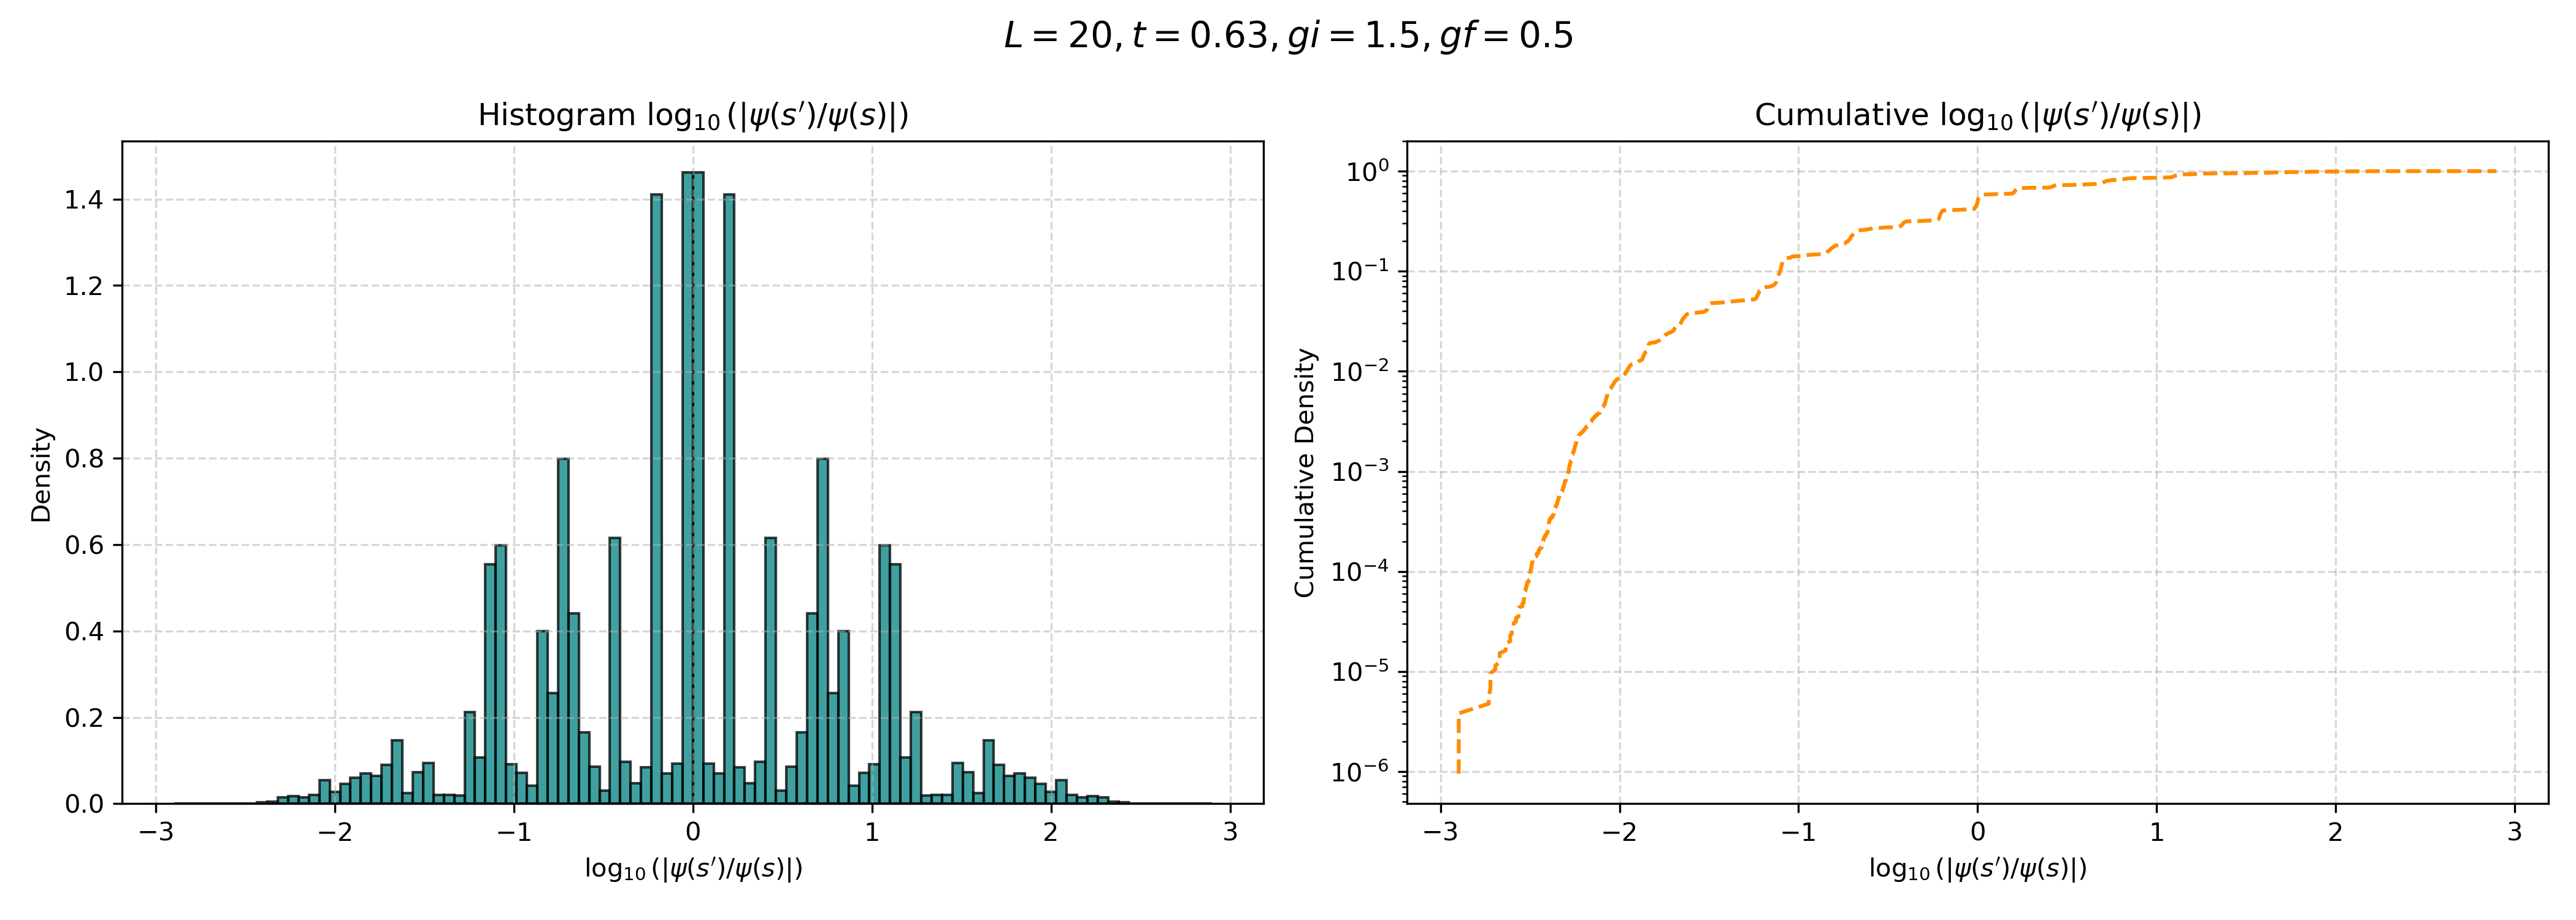
\includegraphics[width=1.0\linewidth]{figures/quench_figures/hist_plot_L20_t63_gi1.50_gf0.50.png}
    \caption{Histogram of amplitude ratios, for $t=0.63$.There is around $20\%$ of the neighboring amplitudes which differ at least in one magnitude order}
    \label{fig:4}
\end{figure}
Figure \ref{fig:4} shows that the histogram has a large tail and  the ratios cover different orders of magnitude.

Now we plot the average order $\langle |A| \rangle$ as a function of time:
\begin{figure}[H]
    \centering
    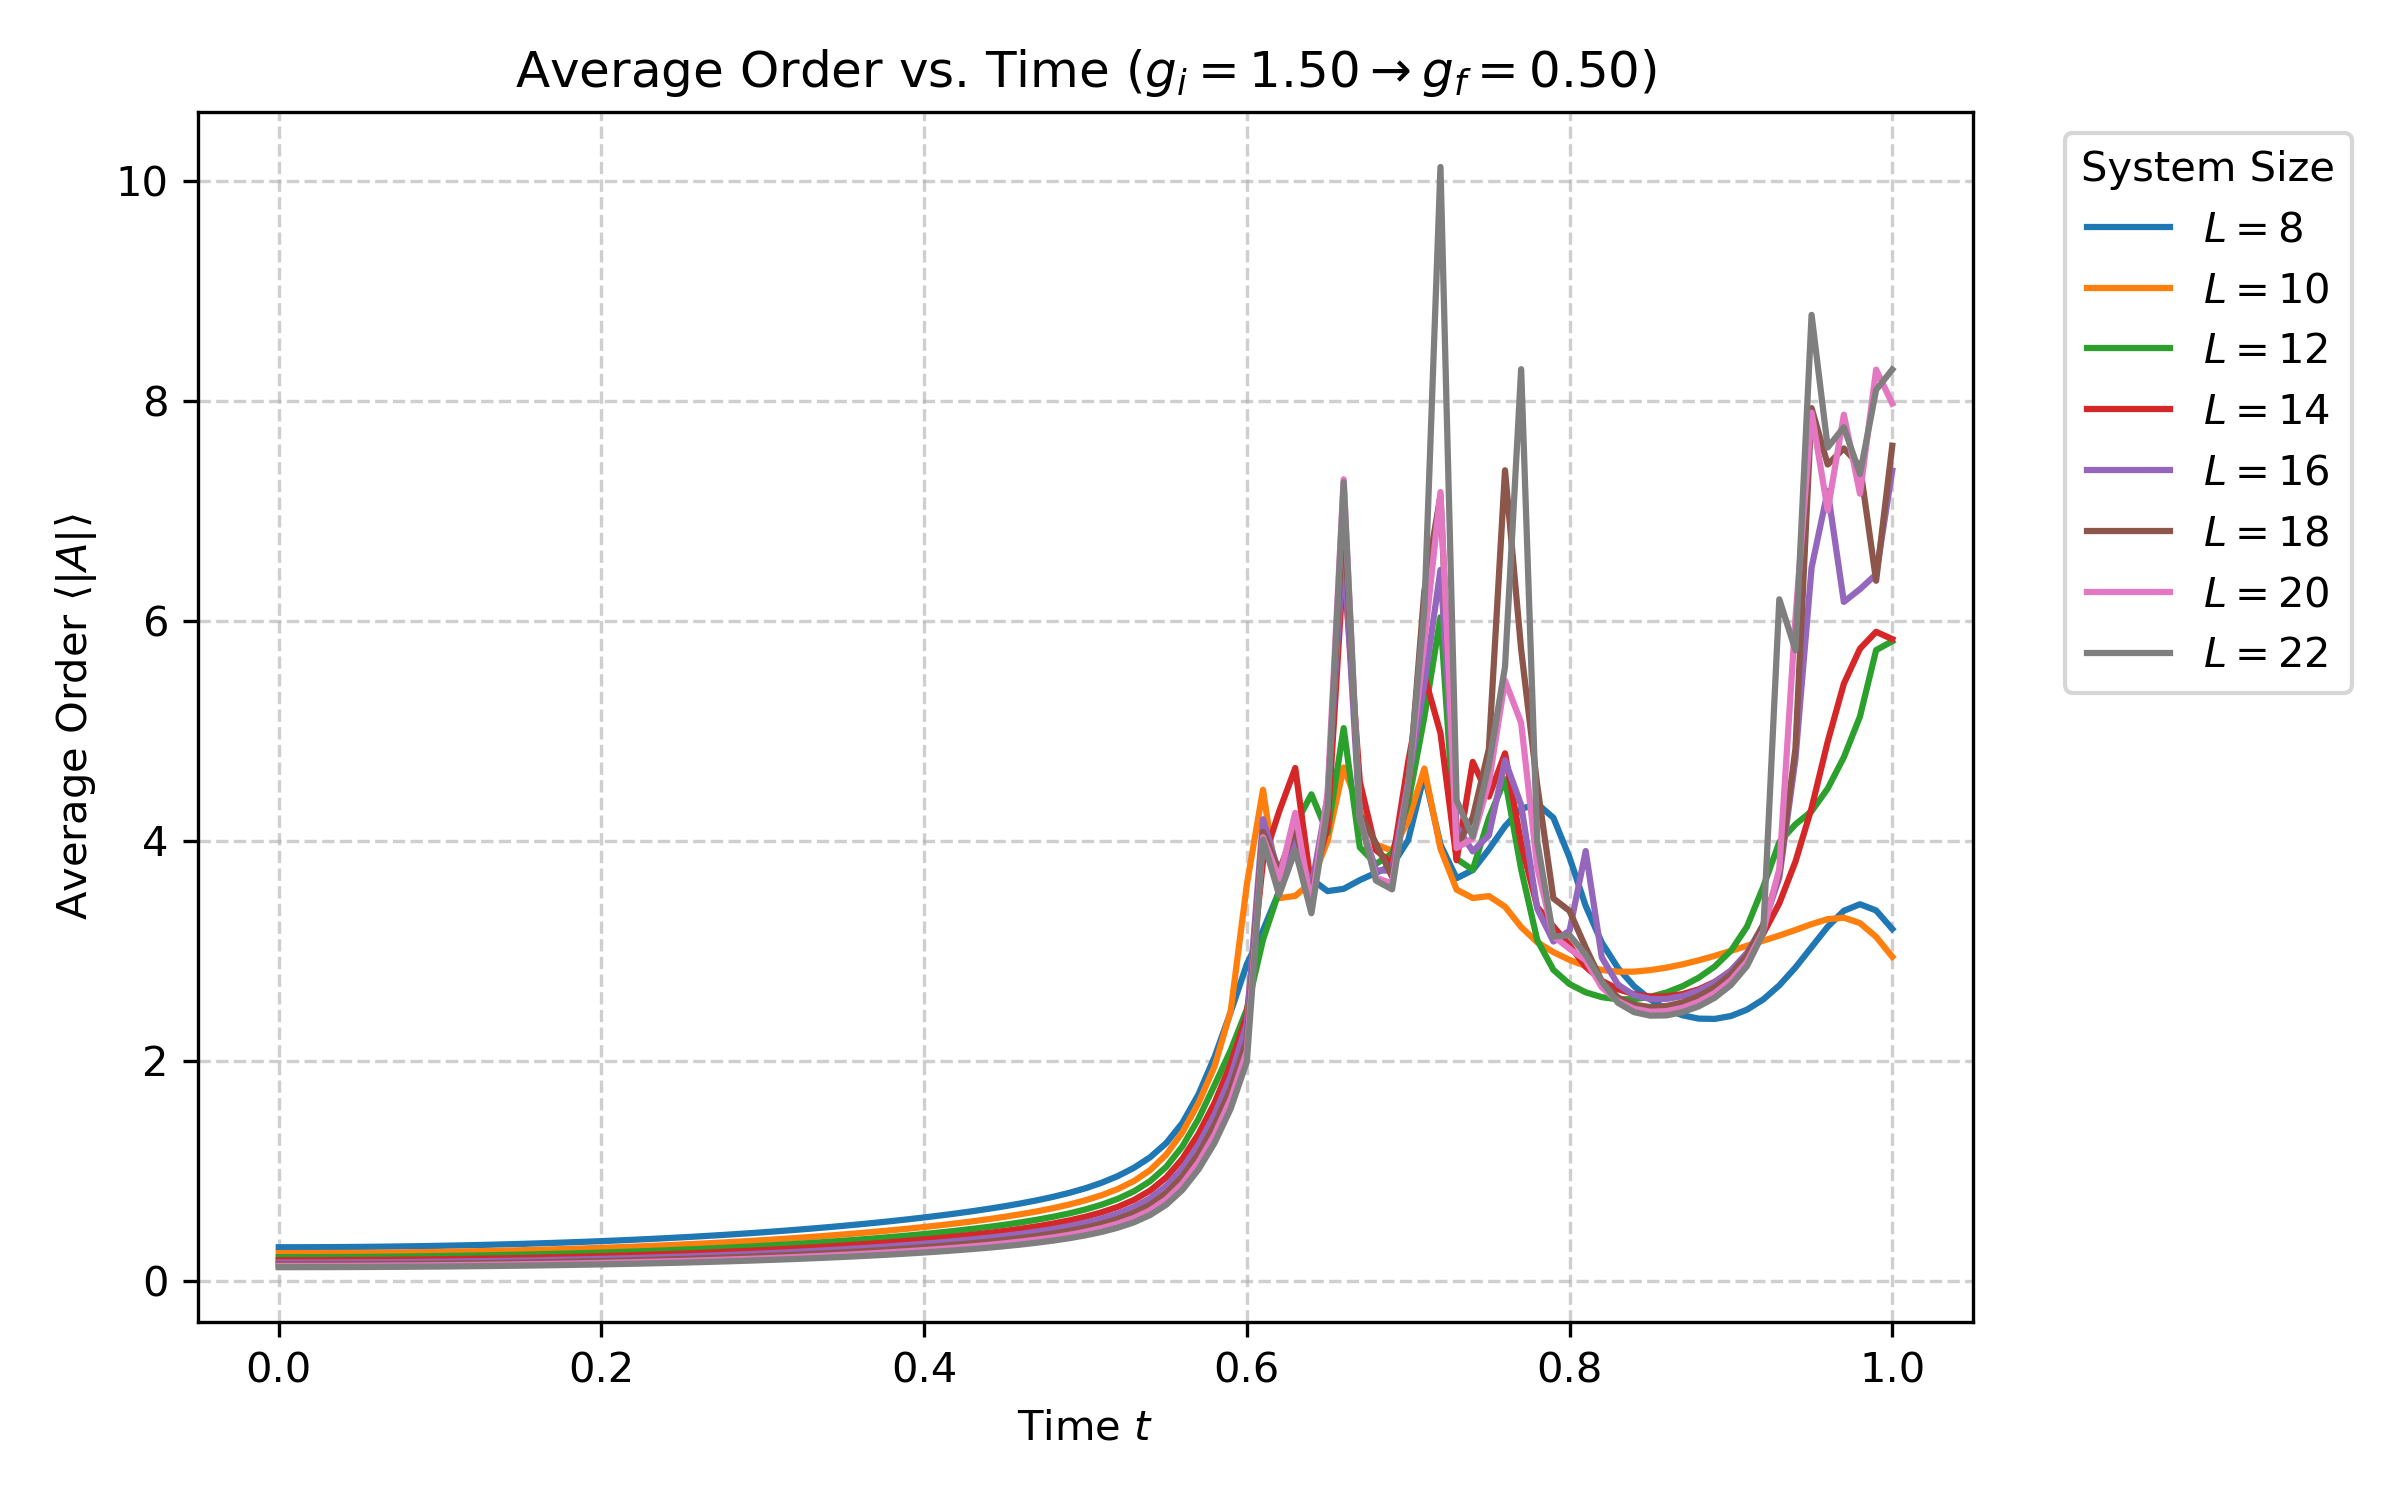
\includegraphics[width=1.0\linewidth]{figures/quench_figures/average_order_plot.png}
    \caption{Average order of the local energy as a function of time.}
    \label{fig:5}
\end{figure}


\textbf{Spectra of the classical network and its properties}


\ref{fig:6} shows the coefficients of the network weighted by the size of their periodic group. We observe a clear transition before crossing the critical time $t^*$ the weights are accumulated in few coefficients, after the transition the weights are spread all over the coefficient space, this drastic behaviour is seen on different compression metrics such as the infidelity \ref{fig:7} and the relative tail remainder \ref{fig:8}.





\ref{fig:7} shows the infidelity of $|\Psi|$ for a continuous truncation of parameters in the network, there is a transition from 

\begin{figure}[H]
    \centering
    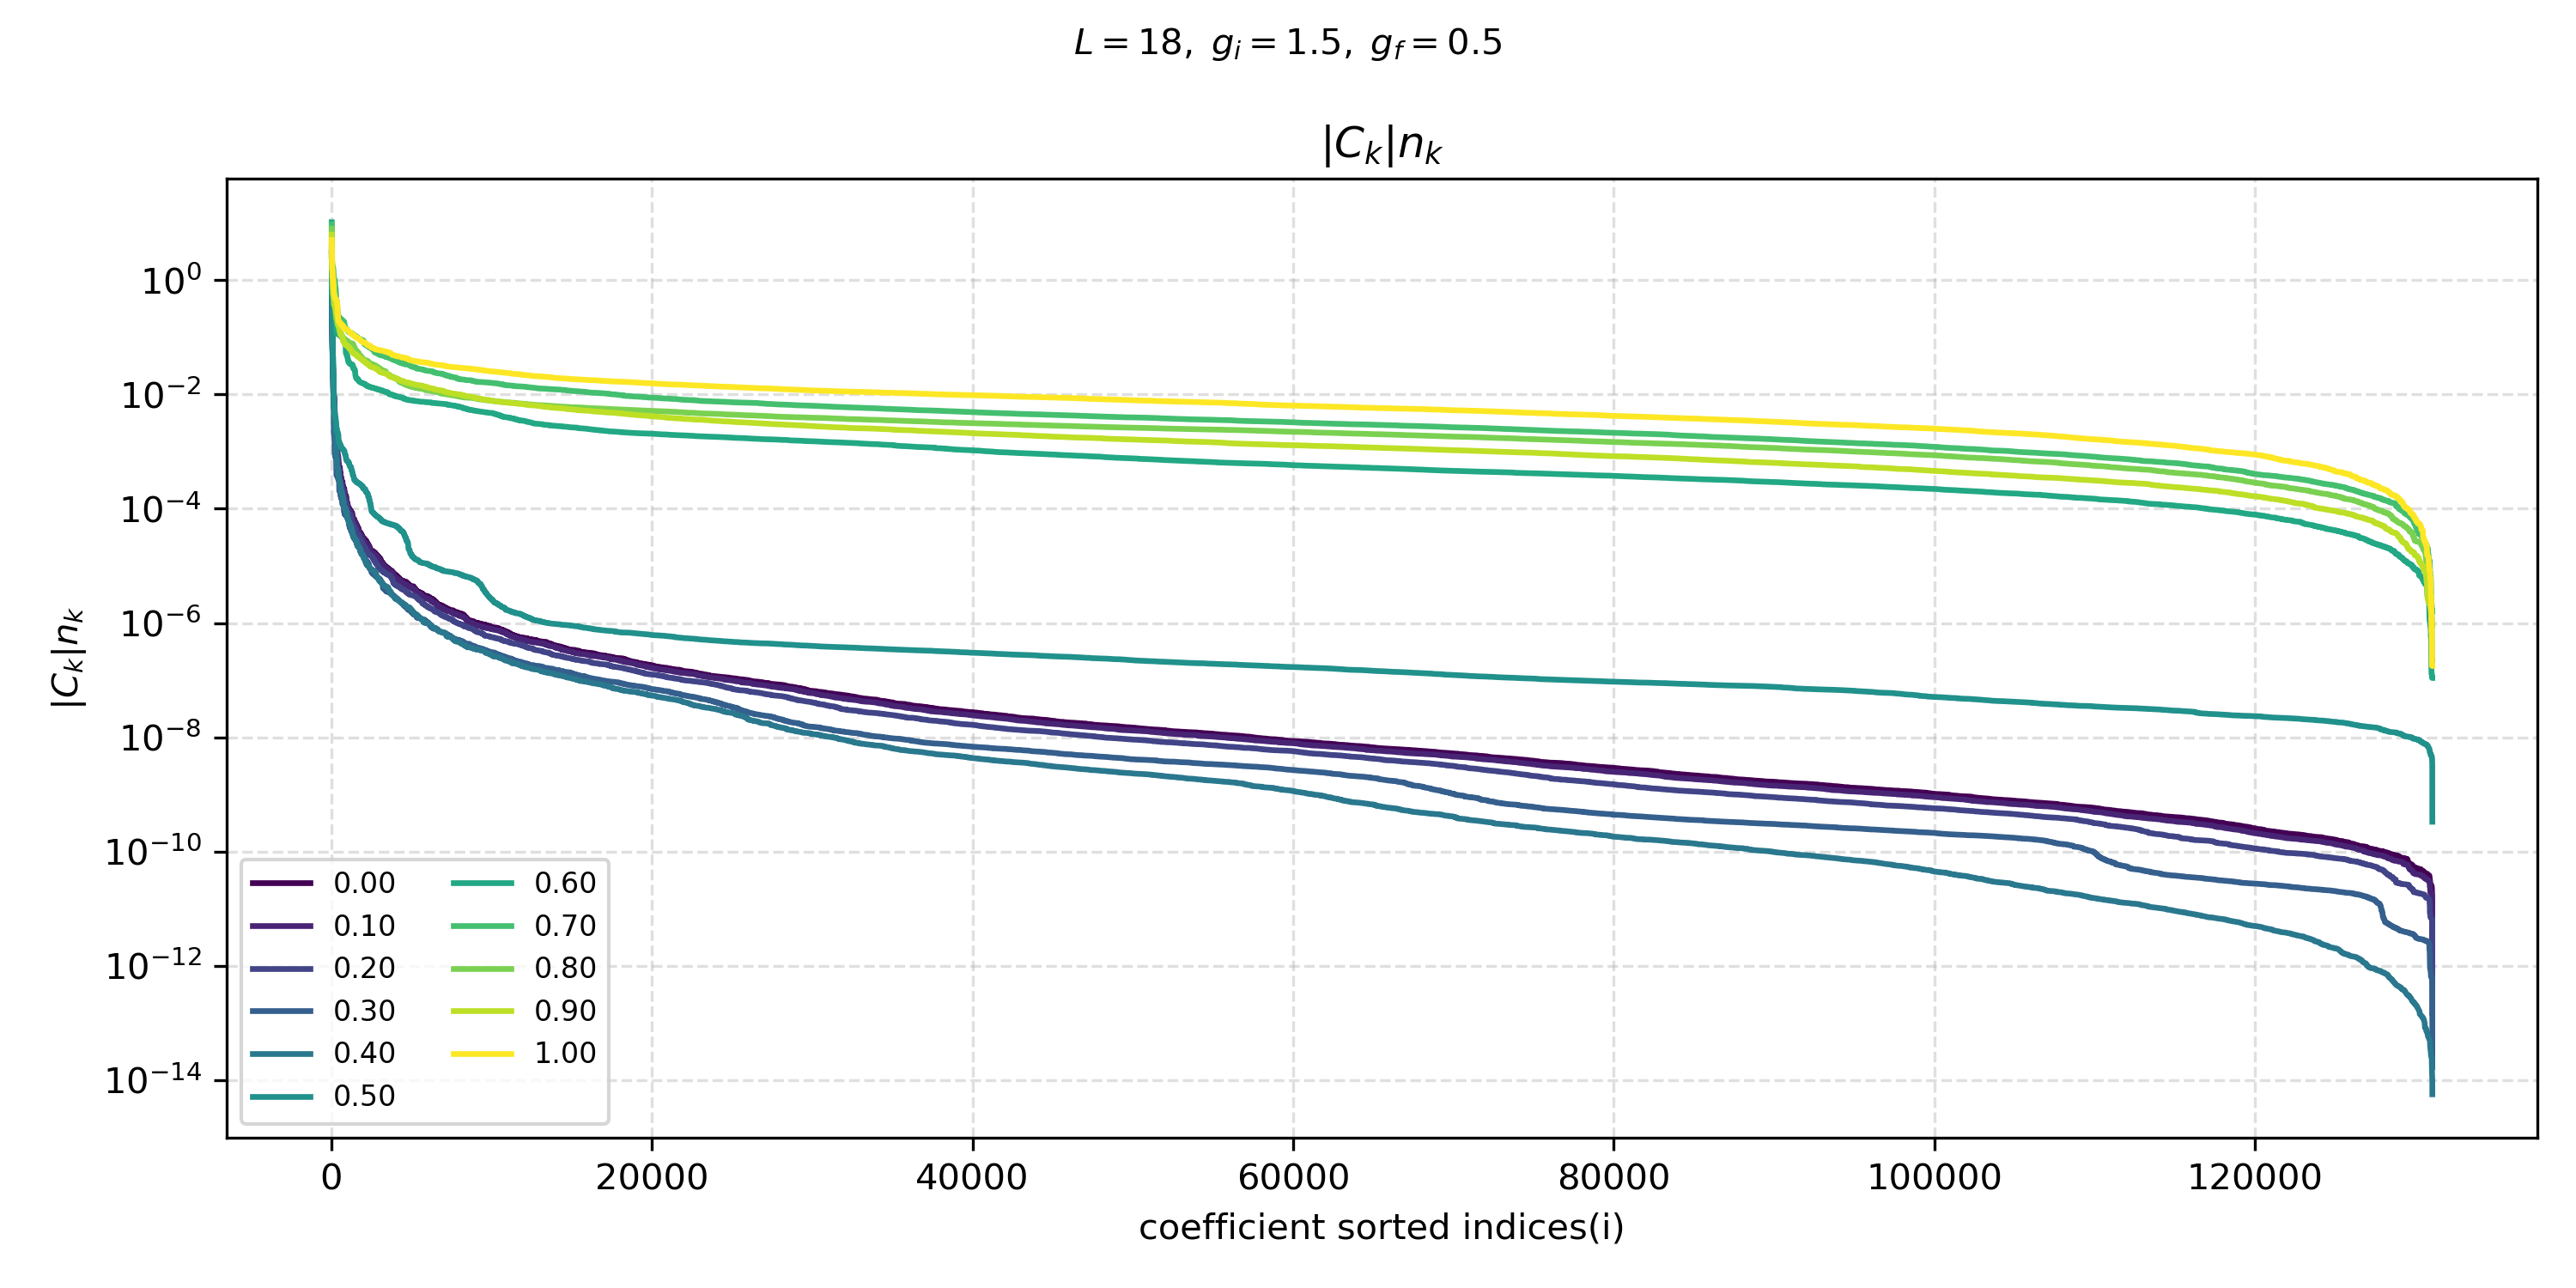
\includegraphics[width=1.0\linewidth]{figures/quench_figures/wht_spectra_L18_gi1.50_gf0.50.png}
    \caption{Spectra of the network coefficients}
    \label{fig:6}
\end{figure}

\begin{figure}[H]
    \centering
    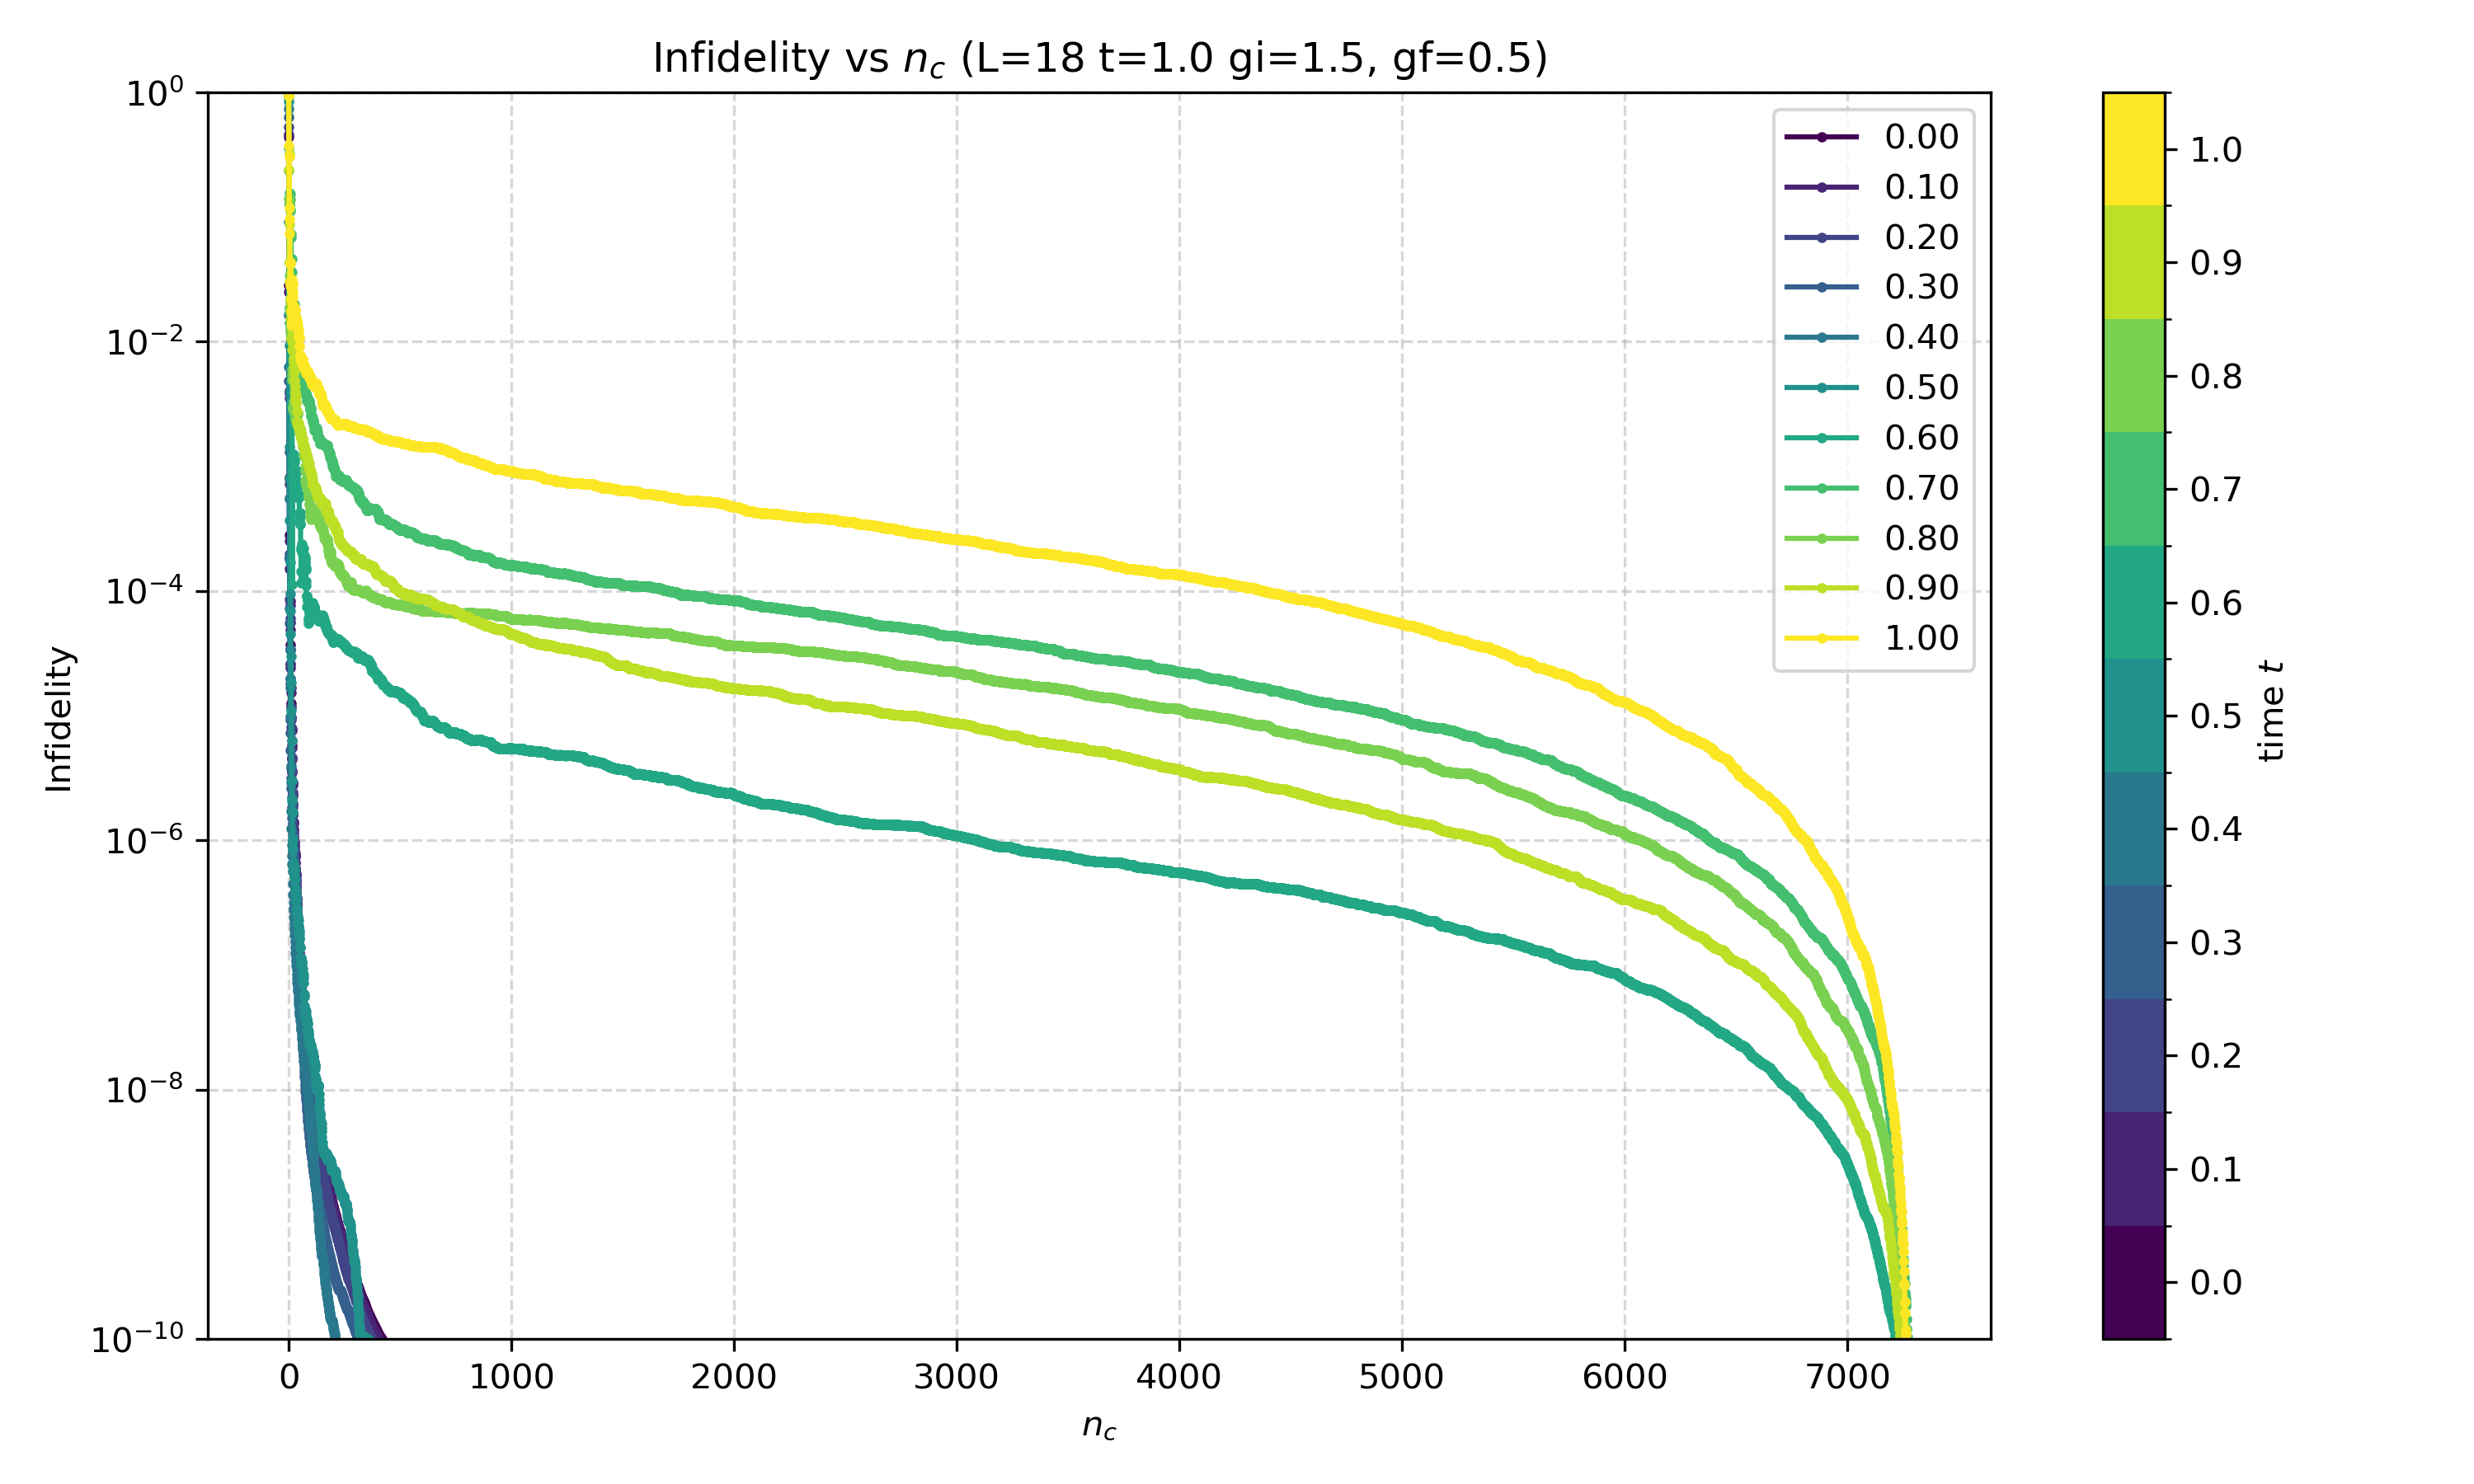
\includegraphics[width=1.0\linewidth]{figures/quench_figures/inf_plot_L18_gi1.5_gf_0.5continuousTrue.png}
    \caption{$I(|\Psi|,|\Psi_{n_c}|)$ for different $n_c$.}
    \label{fig:7}
\end{figure}

\begin{figure}
    \centering
    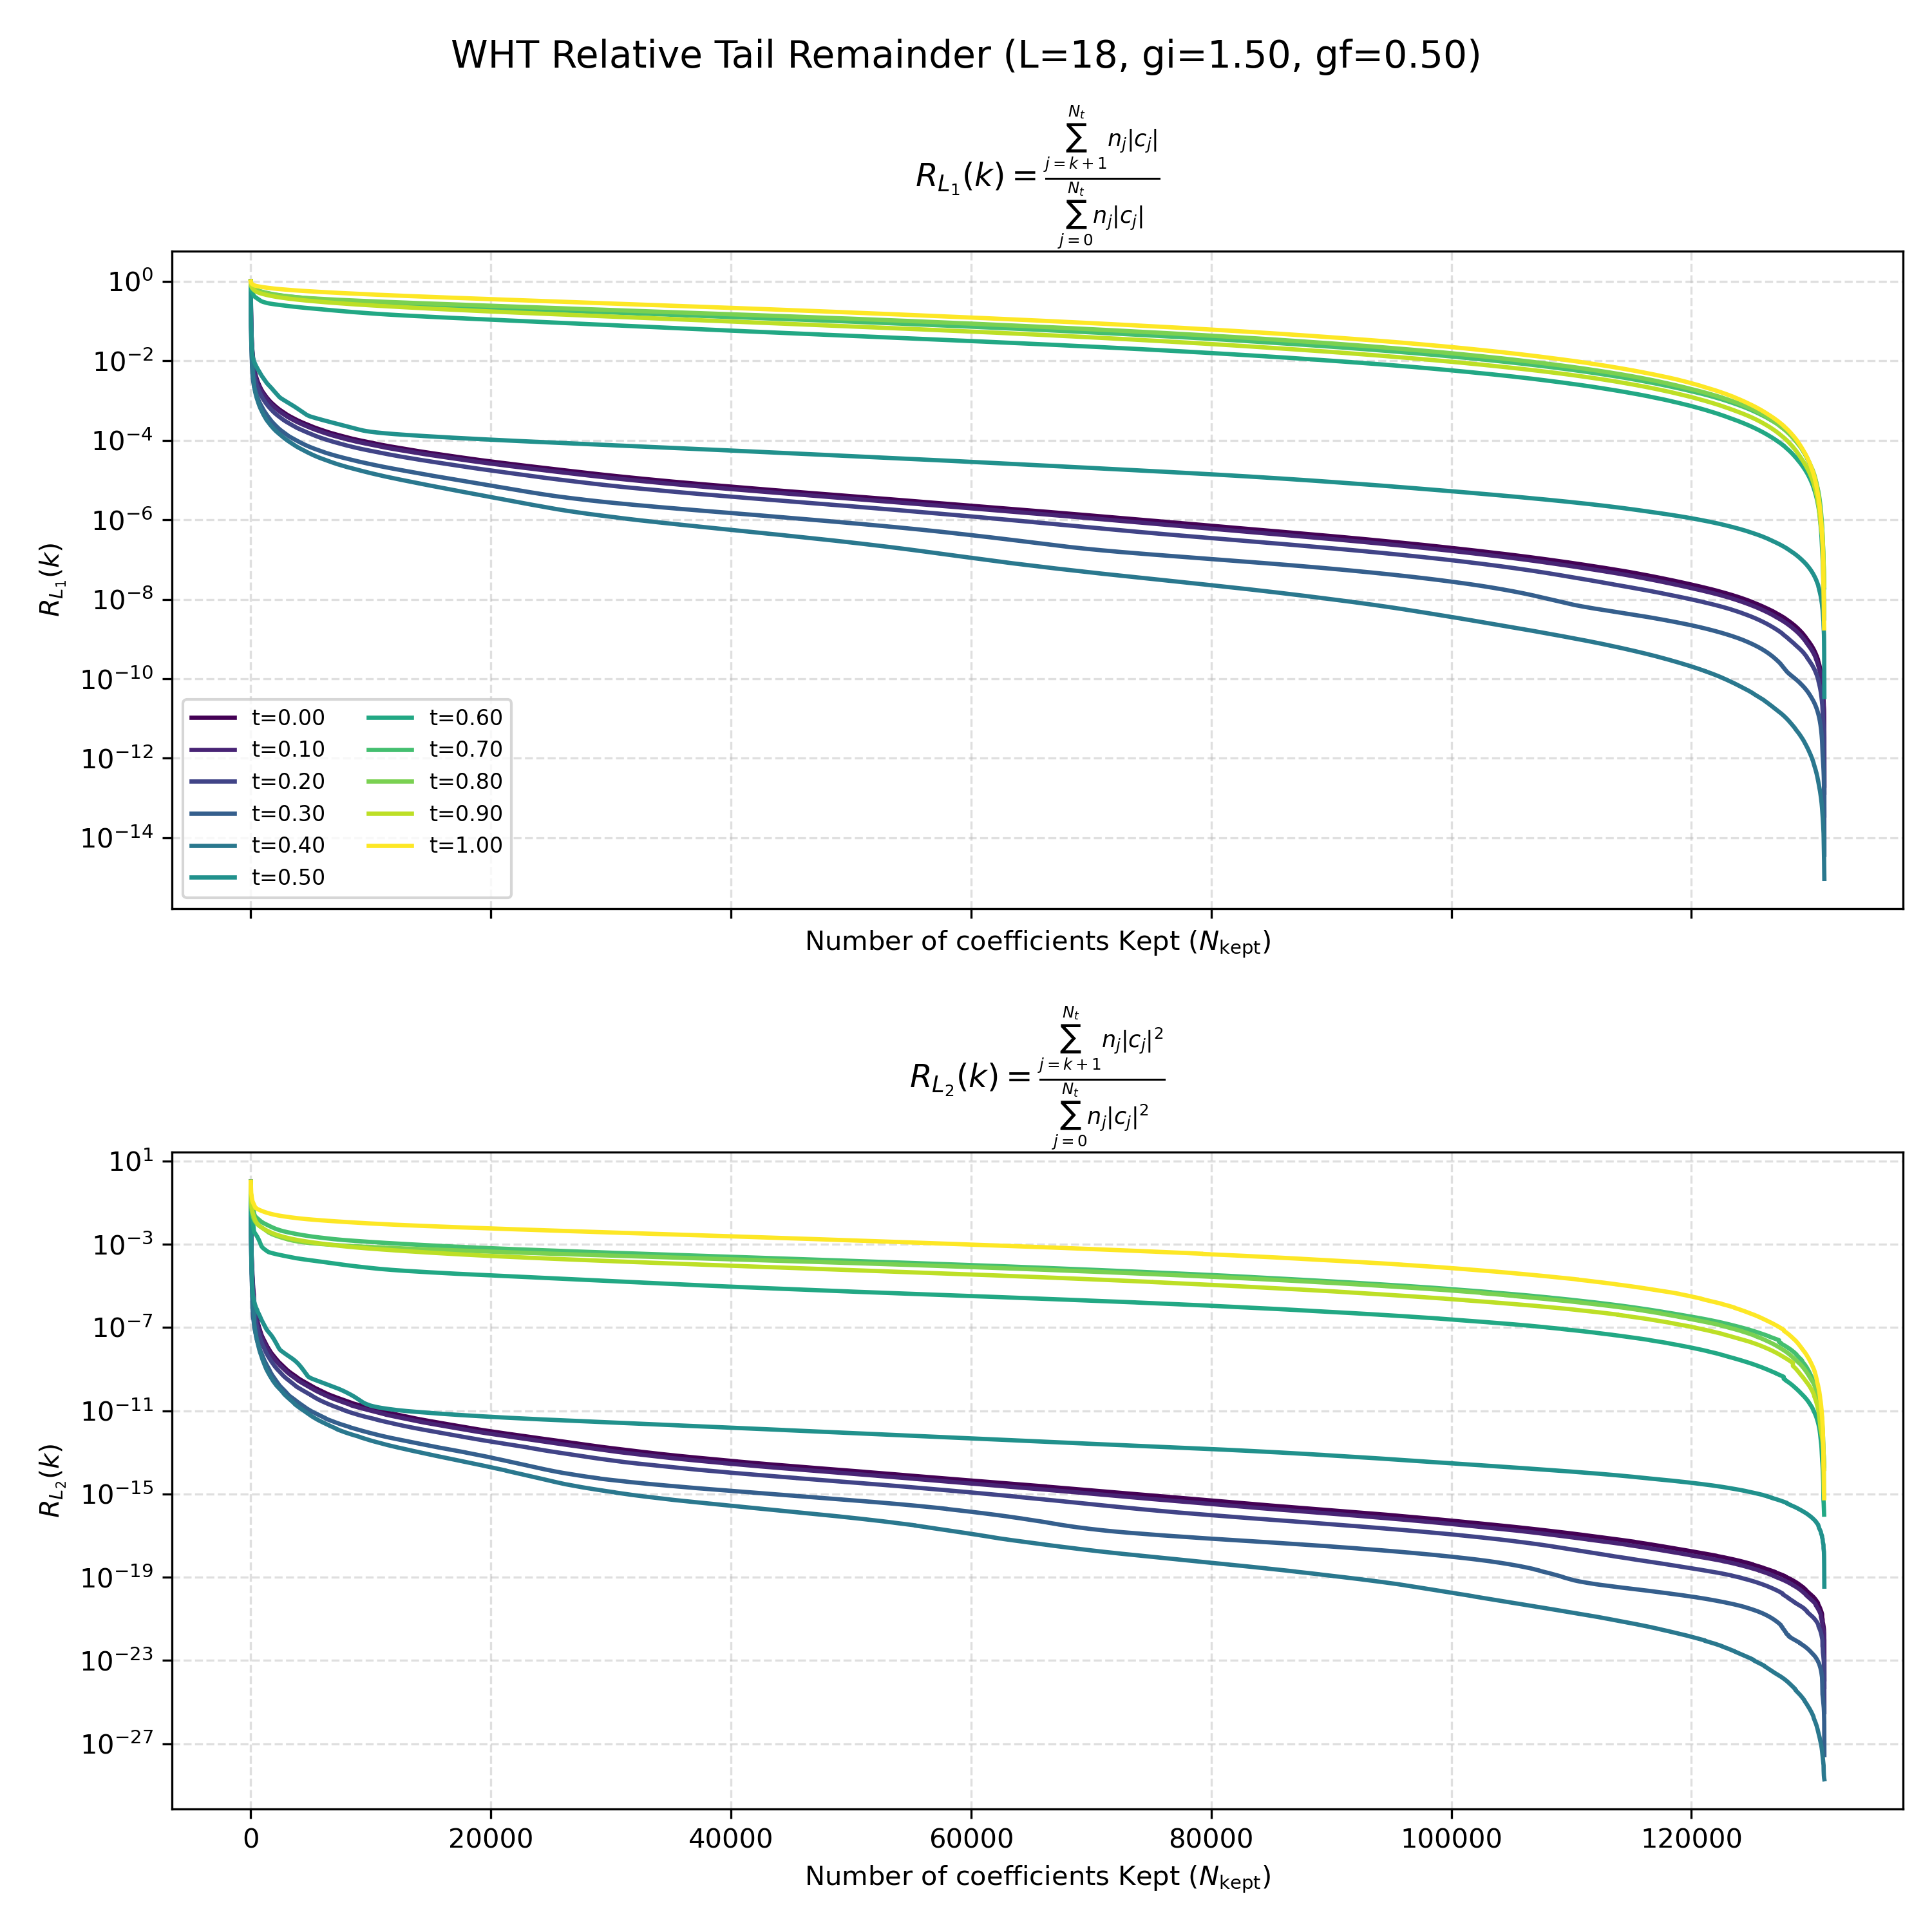
\includegraphics[width=1.0\linewidth]{figures/quench_figures/wht_tail_remainder_both_L18_gi1.50_gf0.50.png}
    \caption{Relative tail remainder for the WHT.}
    \label{fig:8}
\end{figure}







\end{document}